\chapter{Dasar Teori}
\label{chap:dasar teori}

\section{Kriptografi}
Kriptografi merupakan kata berasal dari bahasa Yunani, yaitu kripto dan graphia. Kripto berarti rahasia dan graphia berarti tulisan. Jadi, kriptografi adalah ilmu sekaligus seni untuk untuk menjaga keamanan pesan. Keamanan pesan diperoleh dengan menyandikan pesan menjadi tidak bermakna atau tidak memiliki arti. Zaman sekarang ini, kerahasiaan informasi menjadi suatu hal yang penting. Informasi yang sifatnya rahasia atau personal perlu dilindungi dari orang-orang yang tidak berhak untuk membacanya. Kriptografi digunakan untuk menyamarkan informasi rahasia itu dari orang atau pihak yang tidak berhak untuk membaca atau melihatnya.

Kriptografi memiliki 4 layanan utama:
\begin{enumerate}
	\item Kerahasiaan Data (\textit{data confidentiality})\\
	Layanan ini menjamin bahwa data atau pesan yang dikirimkan tidak diketahui oleh pihak atau orang lain yang tidak berhak untuk membaca atau melihatnya.
	\item Integritas Data (\textit{data integrity})\\
	Layanan yang menjamin data atau pesan yang dikirimkan tidak boleh diubah tanpa seijin pemilik pesan, menjamin keaslian dari data atau pesan yang dikirimkan.
	\item Otentikasi (\textit{authentication})\\
	Layanan yang digunakan untuk menvalidasi identitas seseorang, entitas, atau  asal informasi yang dikirim. Autentikasi dibagi ke dalam 2 jenis dilihat dari subjek yang diotentikasinya, yaitu otentikasi entitas dan otentikasi pesan.
	\item Non-repudiasi (\textit{nonrepudiation})\\
	Layanan yang menjamin bahwa tidak ada penyangkalan baik oleh pengirim atau penerima pesan.
\end{enumerate}

Dalam kriptografi, pesan yang dirahasiakan disebut \textit{plaintext}, sedangkan pesan hasil dari penyandian disebut \textit{ciphertext}. Pesan yang telah disandikan dapat dikembalikan lagi ke pesan aslinya hanya oleh orang yang berhak. Orang yang berhak adalah orang yang mengetahui cara penyandian atau memiliki kunci penyandian. Proses menyandikan \textit{plaintext} menjadi \textit{ciphertext} disebut enkripsi (\textit{encryption}) dan proses mengembalikan \textit{ciphertext} menjadi \textit{plaintext} disebut dekripsi (\textit{decryption}). Dalam proses enkripsi dan dekripsi menggunakan kunci (\textit{key}) yaitu sekumpulan huruf, angka, atau simbol. Kunci ini sifatnya rahasia dan tidak boleh diketahui pihak lain yang tidak berwenang.

%diagram
\begin{figure}[h]
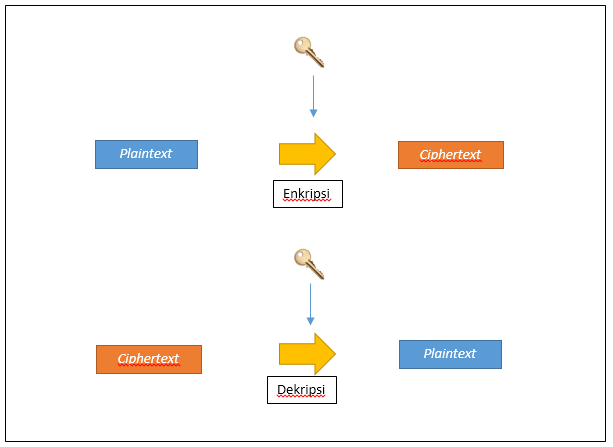
\includegraphics[width=12cm,height=7cm]{Gambar/encryption_decryption}
\centering
\caption{Proses enkripsi dan dekripsi}
\label{fig:prosesenkripsidekripsi}
\end{figure}

Gambar \ref{fig:prosesenkripsidekripsi} ini menunjukkan proses enkripsi dan dekripsi.

Dalam proses enkripsi, \textit{plaintext} akan dipetakan pada fungsi enkripsi \textit{E} menjadi \textit{ciphertext} didasarkan pada kunci \textit{k} seperti notasi di bawah ini:
\begin{displaymath}
	E_k(plaintext) = ciphertext
\end{displaymath}

Kemudian dalam proses dekripsi, untuk mengembalikan \textit{ciphertext} ke \textit{plaintext} maka \textit{ciphertext} akan dipetakan pada fungsi dekripsi \textit{D} didasarkan pada kunci \textit{k} seperti notasi di bawah ini:
\begin{displaymath}
	D_k(ciphertext)=plaintext
\end{displaymath}

Sebagai contoh, \textit{plaintext} yang akan dikirimkan sebagai berikut adalah kriptografi disandikan menjadi \textit{ciphertext} dengan fungsi enkripsi \textit{E} didasarkan pada kunci \textit{k} menjadi:
\begin{displaymath}
E_k(kriptografi)=u8@37md
\end{displaymath}

\noindent \textit{ciphertext} diatas, meskipun tidak dirahasiakan, namun isinya sudah tidak jelas dan tidak dapat dimengerti maksudnya. Hanya orang yang berhak yang dapat mengembalikan \textit{ciphertext} menjadi \textit{plaintext}. Kemudian untuk mengembalikan \textit{ciphertext} ke \textit{plaintext}, \textit{ciphertext} akan dipetakan pada fungsi dekripsi \textit{D} didasarkan pada kunci \textit{k} menjadi:
\begin{displaymath}
D_k(u8@37md)=kriptografi
\end{displaymath}

Algoritma kriptografi ini dibagi menjadi 2 jenis, yaitu:
\begin{enumerate}
	\item Kriptografi kunci simetris (\textit{symmetric key cryptography})\\
		Kriptografi kunci simetris atau penyandian kunci simetris menggunakan hanya satu kunci rahasia. Pengirim pesan mengenkripsi pesan dengan kunci \textit{k}, kemudian penerima pesan juga akan mendekripsi pesan yang diterima dengan kunci \textit{k}. Dalam hal ini, pengirim dan penerima keduanya harus memiliki kunci \textit{k}. Kelemahan dari kriptografi kunci simetris adalah baik pengirim dan penerima harus memiliki kunci yang sama, sehingga pengirim harus mencara cara lain untuk memberitahukan kunci kepada penerima. Contoh algoritma kunci simetris antara lain adalah \textit{Data Encryption Standard} (DES), \textit{Advanced Encryption Standard} (AES), \textit{Twofish}, dan \textit{Blowfish}.
	\item Kriptografi kunci asimetris (\textit{asymmetric key cryptography})\\
	Dalam kriptografi kunci asimetris atau penyandian kunci simetris kunci rahasia yang digunakan ada 2 buah kunci, yaitu kunci publik (\textit{public key}) dan kunci pribadi (\textit{private key}). Kunci publik tidak rahasia dan dapat diketahui secara umum, sedangkan kunci pribadi harus dirahasiakan oleh pengirim pesan. Pengirim pesan akan mengenkripsi pesan yang dikirim dengan kunci publik penerima pesan, kemudian penerima pesan akan mendekripsi pesan menggunakan kunci pribadinya yang hanya diketahui oleh dirinya saja. Contoh algoritma kunci asimetris antara lain adalah Rivest-Shamir-Adleman (RSA), ElGamal, Diffie-Helman, \textit{Digital Signature Algorithm}, dan \textit{Elliptic Curve Digital Signature Algorithm} (ECDSA).
\end{enumerate}

\subsection{\textit{Data Encryption Standard} (DES)}
\textit{Data Encryption Standard} (DES) adalah algoritma kriptografi kunci simetris, yaitu menggunakan kunci yang sama pada proses enkripsi dan dekripsinya. Masukkan dari DES berupa 64-\textit{bit} \textit{plaintext} dan keluarannya berupa 64-\textit{bit} \textit{ciphertext} dengan 64-\textit{bit} kunci. Proses enkripsi terdiri dari 2 proses permutasi, yaitu permutasi awal dan permutasi akhir, dan 16 ronde sandi feistel. Setiap ronde menggunakan kunci 48-\textit{bit} yang berbeda-beda. Kunci dari setiap ronde ini akan didapat dari round-key generator yang berdasarkan pada 64-\textit{bit} kunci sandi. Gambar di bawah ini menunjukkan proses enkripsi dari DES.

%diagram
\begin{figure}[h]
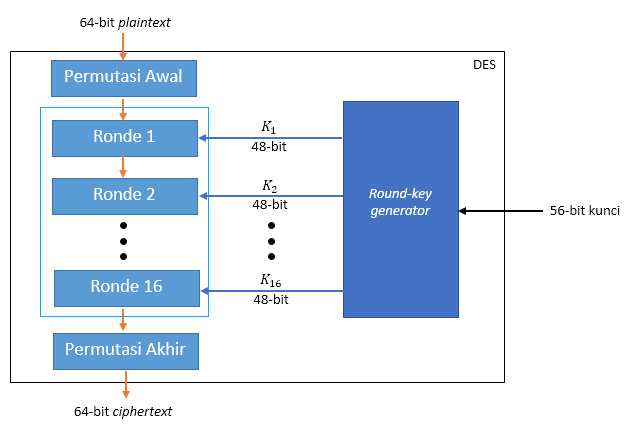
\includegraphics[scale=0.6]{Gambar/DES}%
\centering
\caption{Proses enkripsi dengan DES}
\end{figure}

\subsubsection{Permutasi Awal dan Permutasi Akhir}
Permutasi awal dan akhir dalam DES menggunakan matriks permutasi. Kedua permutasi ini menggunakan 64-\textit{bit} masukan dan matriks yang terdiri 64 nilai yang sudah ditentukan sebelumnya. Matriks ini nilainya selalu sama untuk setiap proses enkripsi dan tidak ada aturan tertentu untuk membuatnya. Tabel \ref{table:awal} dan \ref{table:akhir} menunjukkan matriks permutasi awal dan matriks permutasi akhir.

%diagram
%\begin{figure}[h]
%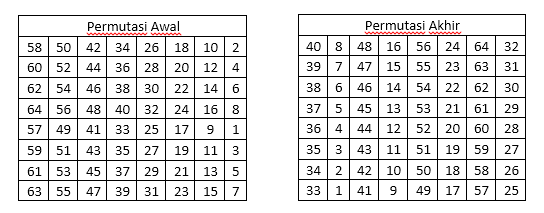
\includegraphics[scale=0.8]{Gambar/permutasi}
%\centering
%\caption{Matriks Permutasi}
%\end{figure}

\begin{table}
	\begin{center}
		\begin{tabular}{|l|l|l|l|l|l|l|l|}
				\hline
				\multicolumn{8}{|c|}{\textit{Permutasi Awal}} \\
				\hline
				58	&	50	&	42	&	34	&	26	&	18	&	10	&	2	\\ \hline
				60	&	52	&	44	&	36	&	28	&	20	&	12	&	4	\\ \hline
				62	&	54	&	46	&	38	&	30	&	22	&	14	&	6	\\ \hline
				64	&	56	&	48	&	40	&	32	&	24	&	16	&	8	\\ \hline
				57	&	49	&	41	&	33	&	25	&	17	&	9	&	1		\\ \hline
				59	&	51	&	43	&	35	&	27	&	19	&	11	&	3	\\ \hline
				61	&	53	&	45	&	37	&	29	&	21	&	13	&	5	\\ \hline
				63	&	55	&	47	&	39	&	31	&	23	&	15	&	7	\\ \hline
		\end{tabular}
	\end{center}
	\caption{Matriks Permutasi Awal}\label{table:awal}
\end{table}

\begin{table}
	\begin{center}
		\begin{tabular}{|l|l|l|l|l|l|l|l|}
				\hline
				\multicolumn{8}{|c|}{\textit{Permutasi Akhir}} \\
				\hline
				40	&	8	&	48	&	16	&	56	&	24	&	64	&	32	\\ \hline
				39	&	7	&	47	&	15	&	55	&	23	&	63	&	31	\\ \hline
				38	&	6	&	46	&	14	&	54	&	22	&	62	&	30	\\ \hline
				37	&	5	&	45	&	13	&	53	&	21	&	61	&	29	\\ \hline
				36	&	4	&	44	&	12	&	52	&	20	&	60	&	28	\\ \hline
				35	&	3	&	43	&	11	&	51	&	19	&	59	&	27	\\ \hline
				34	&	2	&	42	&	10	&	50	&	18	&	58	&	26	\\ \hline
				33	&	1	&	41	&	9		&	49	&	17	&	57	&	25	\\ \hline
		\end{tabular}
	\end{center}
	\caption{Matriks Permutasi Akhir}\label{table:akhir}
\end{table}

Sebagai contoh, \textit{bit} ke-58 dari input akan menjadi \textit{bit} ke-1 pada output permutasi awal, \textit{bit} ke-50 akan menjadi \textit{bit} ke-2 pada output permutasi awal dan seterusnya. Cara yang sama akan diterapkan pada proses permutasi akhir nanti setelah 16 ronde sandi feistel.

%diagram
\begin{figure}[h]
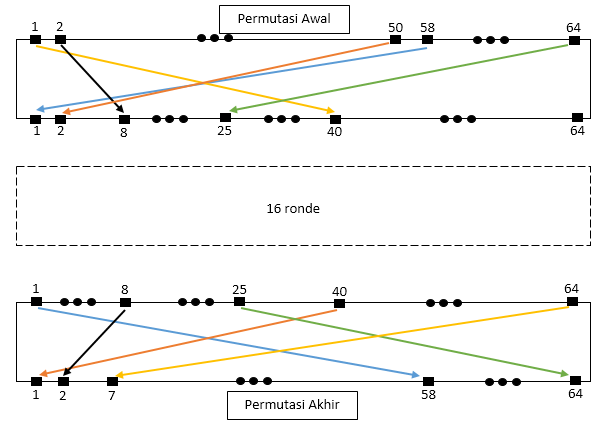
\includegraphics[scale=0.5]{Gambar/proses_permutasi}
\centering
\caption{Proses Permutasi}
\end{figure}

\subsubsection{Ronde}
DES menggunakan 16 ronde. Setiap ronde dari DES adalah sandi feistel yang ditunjukkan pada gambar di bawah.

%diagram
\begin{figure}[h]
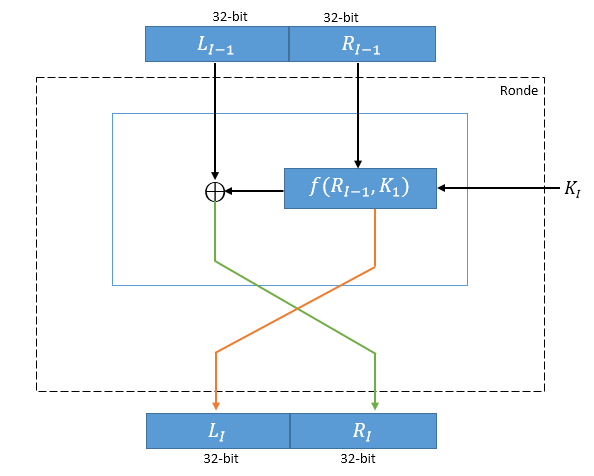
\includegraphics[scale=0.5]{Gambar/round}
\centering
\caption{Ronde dalam DES}
\end{figure}

Setiap ronde menggunakan \begin{math}L_{I-1}\end{math} dan \begin{math}R_{I-1}\end{math} dari ronde sebelumnya (atau dari permutasi awal) dan memrosesnya menjadi \begin{math}L_I\end{math} dan \begin{math}R_I\end{math} untuk nanti dilanjutkan ke proses yang berikutnya (atau permutasi akhir). \begin{math}f(R_{I-1},K_I)\end{math}  merupakan fungsi DES. Plaintext (64-\textit{bit}) akan dibagi 2 menjadi bagian kiri (\textit{L}) dan bagian kanan (\textit{R}). Bagian kanan akan diproses lagi oleh fungsi \begin{math}f(R_{I-1},K_I)\end{math}. Kemudian, hasil dari fungsi \begin{math}f(R_{I-1},K_I)\end{math} akan di XOR dengan bagian kiri. Hasil dari XOR akan menjadi \begin{math}R_I\end{math} dan hasil dari fungsi \begin{math}f(R_{I-1},K_I)\end{math} akan menjadi \begin{math}L_I\end{math}. Pada ronde ke-16 tidak akan terjadi pertukaran antara bagian \begin{math}L_{I-1}\end{math} dan \begin{math}R_{I-1}\end{math}.

\subsubsection{Fungsi DES}
Fungsi DES merupakan inti dari algoritma DES. Fungsi DES menerima masukkan kunci ronde 48-\textit{bit} dan bagian kanan dari plaintext, \begin{math}R_{I-1}\end{math} dan menghasilkan 32-\textit{bit} keluaran. Fungsi ini terdiri dari 4 bagian, yaitu ekspansi \textit{P-box}, operasi XOR, substitusi \textit{S-box}, dan permutasi.

\begin{enumerate}
	\item Ekspansi \textit{P-box}\\
	Pada bagian ini, karena \begin{math}R_{I-1}\end{math} adalah input dengan panjang 32-\textit{bit} dan kunci ronde yang digunakan sepanjang 48-\textit{bit}, maka \begin{math}R_{I-1}\end{math} perlu diekspansi menjadi 48-\textit{bit}. \begin{math}R_{I-1}\end{math} akan dibagi menjadi 8 bagian masing-masing 4-\textit{bit}. Kemudian setiap bagian 4-\textit{bit} ini akan diekspansi menjadi 6-\textit{bit}. Ekspansi ini dilakukan berdasarkan aturan yang sudah ditentukan terlebih dahulu, yaitu
	\begin{enumerate}
		\item \textit{Bit} keluaran ke-2, 3, 4, dan 5 diisi oleh \textit{bit} masukkan ke-1, 2, 3, dan 4.
		\item \textit{Bit} keluaran ke-1 akan diisi oleh \textit{bit} masukkan ke-4 pada bagian sebelumnya.
		\item \textit{Bit} keluaran ke-6 akan diisi oleh \textit{bit} masukkan ke-1 pada bagian sesudahnya.
		\item Untuk bagian ke-1, \textit{bit} keluaran ke-1 akan diisi oleh \textit{bit} ke-32 masukkan.
		\item Untuk bagian ke-8, \textit{bit} keluaran ke-6 akan diisi oleh \textit{bit} ke-1 masukkan.
	\end{enumerate}
	Ekspansi ini dilakukan berdasarkan nilai-nilai yang ada dalam \textit{P-box}. Gambar \ref{fig:expansi} menunjukkan proses ekspansi dan Tabel \ref{table:Pbox} menunjukkan matriks \textit{P-box}.
	
	%diagram
	\begin{figure}[h]
	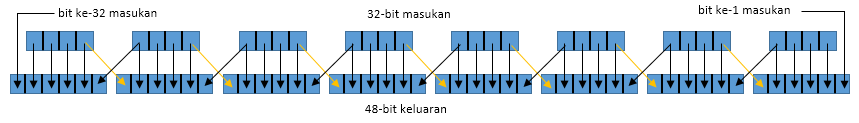
\includegraphics[scale=0.5]{Gambar/expansion_permutation}
	\centering
	\caption{Proses permutasi ekspansi}\label{fig:expansi}
	\end{figure}

\begin{table}
	\begin{center}
		\begin{tabular}{|l|l|l|l|l|l|}
				\hline
				\multicolumn{6}{|c|}{\textit{P-box}} \\
				\hline
				32 	& 1		& 2 	& 3 	& 4 	& 5		\\ \hline
				4 	& 5		& 6 	& 7 	& 8 	& 9		\\ \hline
				8 	& 9		& 10 	& 11 	& 12 	& 13	\\ \hline
				12 	& 13	& 14 	& 15 	& 16 	& 17	\\ \hline
				16 	& 17	& 18 	& 19 	& 20 	& 21	\\ \hline
				20 	& 21	& 22 	& 23 	& 24 	& 25	\\ \hline
				24 	& 25	& 26 	& 27 	& 28 	& 29	\\ \hline
				28 	& 29	& 30 	& 31 	& 32 	& 1		\\ \hline
		\end{tabular}
	\end{center}
	\caption{\textit{P-box}}\label{table:Pbox}
\end{table}

	\item Operasi XOR\\
	Setelah dilakukan ekspansi dengan menggunakan \textit{P-box}, dilakukan operasi XOR antara \begin{math}R_{I-1}\end{math} dengan kunci ronde. Perlu diketahui, bahwa panjang \begin{math}R_{I-1}\end{math} dan kunci ronde sudah sama, yaitu 48-\textit{bit} dan kunci ronde hanya digunakan dalam proses ini saja.

	\item Substitusi \textit{S-box}\\
	DES menggunakan 8 buah \textit{S-box}, masing-masing dengan 6-\textit{bit} masukkan dan 4-\textit{bit} keluaran. Gambar \ref{fig:substitusi_s_box} menunjukkan proses substitusi \textit{S-box} dan Tabel \ref{table:s_box1} menunjukkan \textit{S-box} yang pertama.
	
	%diagram
\begin{figure}[h]
	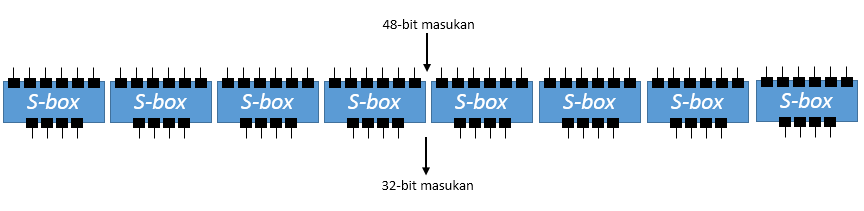
\includegraphics[scale=0.5]{Gambar/S-box}
	\centering
	\caption{Proses substitusi \textit{S-box}}\label{fig:substitusi_s_box}
\end{figure}

\begin{table}
	\begin{center}
		\begin{tabular}{|l|l|l|l|l|l|l|l|l|l|l|l|l|l|l|l|l|}
				\hline
				& 0 & 1	& 2 & 3 & 4 & 5 & 6 & 7 & 8 & 9 & 10 & 11 & 12 & 13 & 14 & 15	\\ \hline
			0 & 14 & 4 & 13 & 1 & 2 & 15 & 11 & 8 & 3 & 10 & 6 & 12 & 5 & 9 & 0 & 7	\\ \hline
			1 & 0 & 15 & 7 & 4 & 14 & 2 & 13 & 10 & 3 & 6 & 12 & 11 & 9 & 5 & 3 & 8	\\ \hline
			2 & 4 & 1 & 14 & 8 & 13 & 6 & 2 & 11 & 15 & 12 & 9 & 7 & 3 & 10 & 5 & 0	\\ \hline
			3 & 15 & 12 & 8 & 2 & 4 & 9 & 1 & 7 & 5 & 11 & 3 & 14 & 10 & 0 & 6 & 13	\\ \hline
		\end{tabular}
	\end{center}
	\caption{\textit{S-box} 1}\label{table:s_box1}
\end{table}

Berikut adalah \textit{S-box} ke-2 sampai dengan \textit{S-box} ke-8.

\begin{table}
	\begin{center}
		\begin{tabular}{|l|l|l|l|l|l|l|l|l|l|l|l|l|l|l|l|l|}
				\hline
				& 0 & 1	& 2 & 3 & 4 & 5 & 6 & 7 & 8 & 9 & 10 & 11 & 12 & 13 & 14 & 15	\\ \hline
			0 & 15 & 1 & 8 & 14 & 6 & 11 & 3 & 4 & 9 & 7 & 2 & 13 & 12 & 0 & 5 & 10	\\ \hline
			1 & 3 & 13 & 4 & 7 & 15 & 2 & 8 & 12 & 12 & 0 & 1 & 10 & 6 & 9 & 11 & 5	\\ \hline
			2 & 0 & 14 & 7 & 11 & 10 & 4 & 13 & 1 & 5 & 8 & 12 & 6 & 9 & 3 & 2 & 15	\\ \hline
			3 & 13 & 8 & 10 & 1 & 3 & 15 & 4 & 2 & 11 & 6 & 7 & 12 & 0 & 5 & 14 & 9	\\ \hline
		\end{tabular}
	\end{center}
	\caption{\textit{S-box} 2}\label{table:s_box2}
\end{table}

\begin{table}
	\begin{center}
		\begin{tabular}{|l|l|l|l|l|l|l|l|l|l|l|l|l|l|l|l|l|}
				\hline
				& 0 & 1	& 2 & 3 & 4 & 5 & 6 & 7 & 8 & 9 & 10 & 11 & 12 & 13 & 14 & 15	\\ \hline
			0 & 10 & 0 & 9 & 14 & 6 & 3 & 15 & 5 & 1 & 13 & 12 & 7 & 11 & 4 & 2 & 8	\\ \hline
			1 & 13 & 7 & 0 & 9 & 3 & 4 & 6 & 10 & 2 & 8 & 5 & 14 & 12 & 11 & 15 & 1	\\ \hline
			2 & 13 & 6 & 4 & 9 & 8 & 15 & 3 & 0 & 11 & 1 & 2 & 12 & 5 & 10 & 14 & 7	\\ \hline
			3 & 1 & 10 & 13 & 0 & 6 & 9 & 8 & 7 & 4 & 15 & 14 & 3 & 11 & 5 & 2 & 12	\\ \hline
		\end{tabular}
	\end{center}
	\label{table:s_box3}
	\caption{\textit{S-box} 3}
\end{table}

\begin{table}
	\begin{center}
		\begin{tabular}{|l|l|l|l|l|l|l|l|l|l|l|l|l|l|l|l|l|}
				\hline
				& 0 & 1	& 2 & 3 & 4 & 5 & 6 & 7 & 8 & 9 & 10 & 11 & 12 & 13 & 14 & 15	\\ \hline
			0 & 7	&	13	&	14	&	3	&	0	&	6	&	9	&	10	&	1	&	2	&	8	&	5	&	11	&	12	&	4	&	15	\\ \hline
			1 & 13	&	8	&	11	&	5	&	6	&	15	&	0	&	3	&	4	&	7	&	2	&	12	&	1	&	10	&	14	&	9	\\ \hline
			2 & 10	&	6	&	9	&	0	&	12	&	11	&	7	&	13	&	15	&	1	&	3	&	14	&	5	&	2	&	8	&	4	\\ \hline
			3 & 3	&	15	&	0	&	6	&	10	&	1	&	13	&	8	&	9	&	4	&	5	&	11	&	12	&	7	&	2	&	14	\\ \hline
		\end{tabular}
	\end{center}
	\label{table:s_box4}
	\caption{\textit{S-box} 4}
\end{table}

\begin{table}
	\begin{center}
		\begin{tabular}{|l|l|l|l|l|l|l|l|l|l|l|l|l|l|l|l|l|}
				\hline
				& 0 & 1	& 2 & 3 & 4 & 5 & 6 & 7 & 8 & 9 & 10 & 11 & 12 & 13 & 14 & 15	\\ \hline
			0	&	2	&	12	&	4	&	1	&	7	&	10	&	11	&	6	&	8	&	5	&	3	&	15	&	13	&	0	&	14	&	9	\\ \hline
			1	&	14	&	11	&	2	&	12	&	4	&	7	&	13	&	1	&	5	&	0	&	15	&	10	&	3	&	9	&	8	&	6	\\ \hline
			2	&	4	&	2	&	1	&	11	&	10	&	13	&	7	&	8	&	15	&	9	&	12	&	5	&	6	&	3	&	0	&	14	\\ \hline
			3	&	11	&	8	&	12	&	7	&	1	&	14	&	2	&	13	&	6	&	15	&	0	&	9	&	10	&	4	&	5	&	3	\\ \hline
		\end{tabular}
	\end{center}
	\label{table:s_box5}
	\caption{\textit{S-box} 5}
\end{table}

\begin{table}
	\begin{center}
		\begin{tabular}{|l|l|l|l|l|l|l|l|l|l|l|l|l|l|l|l|l|}
				\hline
				& 0 & 1	& 2 & 3 & 4 & 5 & 6 & 7 & 8 & 9 & 10 & 11 & 12 & 13 & 14 & 15	\\ \hline
			0	&	12	&	1	&	10	&	15	&	9	&	2	&	6	&	8	&	0	&	13	&	3	&	4	&	14	&	7	&	5	&	11	\\ \hline
			1	&	10	&	15	&	4	&	2	&	7	&	12	&	9	&	5	&	6	&	1	&	13	&	14	&	0	&	11	&	3	&	8	\\ \hline
			2	&	9	&	14	&	15	&	5	&	2	&	8	&	12	&	3	&	7	&	0	&	4	&	10	&	1	&	13	&	11	&	6	\\ \hline
			3	&	4	&	3	&	2	&	12	&	9	&	5	&	15	&	10	&	11	&	14	&	1	&	7	&	6	&	0	&	8	&	13	\\ \hline
		\end{tabular}
	\end{center}
	\label{table:s_box6}
	\caption{\textit{S-box} 6}
\end{table}

\begin{table}
	\begin{center}
		\begin{tabular}{|l|l|l|l|l|l|l|l|l|l|l|l|l|l|l|l|l|}
				\hline
					& 0 & 1	& 2 & 3 & 4 & 5 & 6 & 7 & 8 & 9 & 10 & 11 & 12 & 13 & 14 & 15	\\ \hline
				0	&	4	&	11	&	2	&	14	&	15	&	0	&	8	&	13	&	3	&	12	&	9	&	7	&	5	&	10	&	6	&	1	\\ \hline
				1	&	13	&	0	&	11	&	7	&	4	&	9	&	1	&	10	&	14	&	3	&	5	&	12	&	2	&	15	&	8	&	6	\\ \hline
				2	&	1	&	4	&	11	&	13	&	12	&	3	&	7	&	14	&	10	&	15	&	6	&	8	&	0	&	5	&	9	&	2	\\ \hline
				3	&	6	&	11	&	13	&	8	&	1	&	4	&	10	&	7	&	9	&	5	&	0	&	15	&	14	&	2	&	3	&	12	\\ \hline
		\end{tabular}
	\end{center}
	\label{table:s_box7}
	\caption{\textit{S-box} 7}
\end{table}

\begin{table}
	\begin{center}
		\begin{tabular}{|l|l|l|l|l|l|l|l|l|l|l|l|l|l|l|l|l|}
				\hline
				& 0 & 1	& 2 & 3 & 4 & 5 & 6 & 7 & 8 & 9 & 10 & 11 & 12 & 13 & 14 & 15	\\ \hline
			0	&	13	&	2	&	8	&	4	&	6	&	15	&	11	&	1	&	10	&	9	&	3	&	14	&	5	&	0	&	12	&	7	\\ \hline
			1	&	1	&	15	&	13	&	8	&	10	&	3	&	7	&	4	&	12	&	5	&	6	&	11	&	0	&	14	&	9	&	2	\\ \hline
			2	&	7	&	11	&	4	&	1	&	9	&	12	&	14	&	2	&	0	&	6	&	10	&	13	&	15	&	3	&	5	&	8	\\ \hline
			3	&	2	&	1	&	14	&	7	&	4	&	10	&	8	&	13	&	15	&	12	&	9	&	0	&	3	&	5	&	6	&	11	\\ \hline
		\end{tabular}
	\end{center}
	\label{table:s_box8}
	\caption{\textit{S-box} 8}
\end{table}

Pada bagian ini, akan dilakukan operasi substitusi berdasarkan aturan pada \textit{S-box}. Setiap \textit{S-box} adalah matriks berukuran 4x16 (4 baris, 16 kolom). Setiap isi dari \textit{S-box} akan berbeda-beda. Kombinasi biner dari \textit{bit} ke-1 dan ke-6 masukan menunjukkan posisi baris yang akan dipilih dan kombinasi biner dari \textit{bit} masukan sisanya menunjukkan posisi kolom yang akan dipilih. Setelah itu, angka yang ditunjuk oleh baris dan kolom kombinasi biner ini akan diubah juga menjadi biner.

	Sebagai contoh, misalkan masukan untuk \textit{S-box} diatas adalah 110011. Maka, baris yang dipilih adalah 11 dalam biner dan 3 dalam desimal dan kolom yang dipilih adalah 1001 dalam biner dan 9 dalam desimal. Berarti, nilai yang didapat berdasarkan \textit{S-box} diatas adalah 11 dan dalam biner adalah 1011. Maka, keluaran dari 110011 adalah 1011.

	\item Permutasi\\
Bagian terakhir dari fungsi DES adalah permutasi langsung dengan masukan 32-\textit{bit} dan keluaran 32-\textit{bit}. Proses nya sama dengan permutasi yang dilakukan pada awal proses enkripsi tetapi ukuran matriks permutasi 4x8 (4 baris, 8 kolom). Gambar di bawah ini menunjukkan matriks permutasi langsung.

\begin{table}
	\begin{center}
		\begin{tabular}{|l|l|l|l|l|l|l|l|}
				\hline
			16	&	7	&	20	&	21	&	29	&	12	&	28	&	17	\\ \hline
			1	&	15	&	23	&	26	&	5	&	18	&	31	&	10		\\ \hline
			2	&	8	&	24	&	14	&	32	&	27	&	3	&	9				\\ \hline
			19	&	13	&	30	&	6	&	22	&	11	&	4	&	25	\\ \hline
		\end{tabular}
	\end{center}
	\caption{Matriks Permutasi Langsung}\label{table:permutasi_langsung}
\end{table}

%diagram
%\begin{figure}[ht]
	%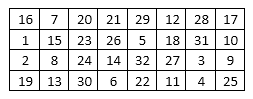
\includegraphics[scale=0.5]{Gambar/straight_permutation}
	%\centering
	%\caption{Matriks Permutasi Langsung}\label{fig:permutasi_langsung}
%\end{figure}

Sama halnya seperti proses permutasi yang dilakukan di awal enkripsi, angka 16 menunjukkan bahwa \textit{bit} ke-16 masukan akan menjadi \textit{bit} ke-1 keluaran, \textit{bit} ke-7 masukan akan menjadi \textit{bit} ke-2 keluaran, dan seterusnya.
\end{enumerate}

\subsection{Pembangunan Kunci Ronde}
Pembangunan kunci ronde adalah algoritma untuk membentuk kunci yang akan digunakan pada setiap ronde. Pembangunan kunci ronde akan menghasilkan 16 kunci masing-masing dengan panjang 48-\textit{bit} dari masukan 56-\textit{bit} kunci sandi. Tetapi, sebenarnya panjang sandi kunci ini adalah 64-\textit{bit} dengan 8-\textit{bit} \textit{parity bit}. \textit{Parity bit} akan dihilangkan sebelum proses pembangkitan kunci sandi 56-\textit{bit}. Proses pembangkitan kunci sandi 56-\textit{bit} bisa dilihat pada gambar di bawah.

%diagram
\begin{figure}[h]
	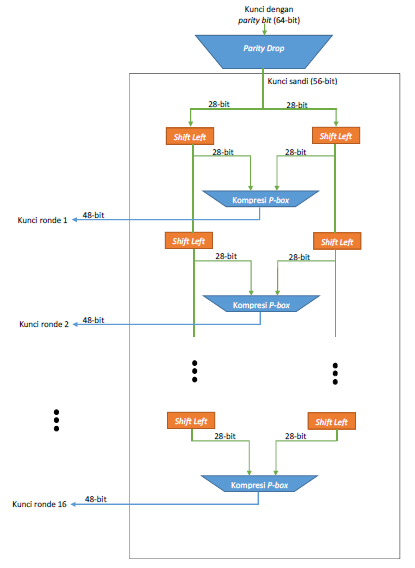
\includegraphics[scale=0.8]{Gambar/key_generation2}
	\centering
	\caption{\textit{Round-Key Generator}}
\end{figure}

\subsubsection{\textit{Parity Drop}}
Proses yang dilakukan sebelum pembangkitan kunci sandi adalah penghilangan \textit{parity bit} pada kunci sandi 64-\textit{bit}. Bit yang dihilangkan adalah \textit{bit} ke-8, 16, 24, 32, ..., 64 sehingga hasil akhirnya adalah 56-\textit{bit} sandi kunci yang nanti kunci ini akan digunakan untuk membuat kunci setiap ronde. Matriks permutasi yang digunakan pada proses ini ditunjukkan pada gambar di bawah.

\begin{table}
	\begin{center}
		\begin{tabular}{|l|l|l|l|l|l|l|l|}
				\hline
				57	&	49	&	41	&	33	&	25	&	17	&	9	&	1	\\ \hline
				58	&	50	&	42	&	34	&	26	&	18	&	10	&	2	\\ \hline
				59	&	51	&	43	&	35	&	27	&	19	&	11	&	3	\\ \hline
				60	&	52	&	44	&	36	&	63	&	55	&	47	&	39	\\ \hline
				31	&	23	&	15	&	7	&	62	&	54	&	46	&	38	\\ \hline
				30	&	22	&	14	&	6	&	61	&	53	&	45	&	37	\\ \hline
				29	&	21	&	13	&	5	&	28	&	20	&	12	&	4	\\ \hline
		\end{tabular}
	\end{center}
	\label{table:parity_drop}
	\caption{Matriks Permutasi untuk \textit{Parity Drop}}
\end{table}

%diagram
%\begin{figure}[ht]
	%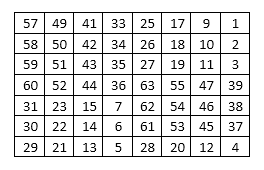
\includegraphics[scale=0.8]{Gambar/parity_drop}
	%\centering
	%\caption{Matriks permutasi untuk \textit{Parity drop}}
%\end{figure}

\subsubsection{\textit{Shift Left}}
Pada tahap ini, kunci yang akan dibentuk akan dipisah menjadi 2 bagian masing-masing 28-\textit{bit}. Setiap bagian akan digeser ke arah kiri secara sirkular sebanyak 1 atau 2 \textit{bit}. Ronde ke-1, 2, 9, dan 16 akan digeser sebanyak 1 \textit{bit}, selain itu hanya akan digeser sebanyak 2 \textit{bit}. Kemudian, kedua bagian ini akan disatukan kembali menjadi satu bagian dengan panjang 56-\textit{bit}.

\subsubsection{Kompresi \textit{P-box}}
\label{sssec:kompresi_Pbox}
Kompresi dengan \textit{P-box} adalah tahap permutasi untuk mengubah kunci 56-\textit{bit} menjadi 48-\textit{bit} agar bisa digunakan sebagai ronde kunci. Kompresi ini menggunakan matriks permutasi \textit{P-box} dengan ukuran 6x8 seperti Tabel \ref{table:kompresi_p}.

\begin{table}
	\begin{center}
		\begin{tabular}{|l|l|l|l|l|l|l|l|}
				\hline
				14	&	17	&	11	&	24	&	1	&	5	&	3	&	28	\\ \hline
				15	&	6	&	21	&	10	&	23	&	19	&	12	&	4	\\ \hline
				26	&	8	&	16	&	7	&	27	&	20	&	13	&	2	\\ \hline
				41	&	52	&	31	&	37	&	47	&	55	&	30	&	40	\\ \hline
				51	&	45	&	33	&	48	&	44	&	49	&	39	&	56	\\ \hline
				32	&	29	&	36	&	50	&	42	&	46	&	53	&	34	\\ \hline
		\end{tabular}
	\end{center}
	\label{table:kompresi_p}
	\caption{Matriks kompresi \textit{P-box}}
\end{table}

%diagram
%\begin{figure}[ht]
	%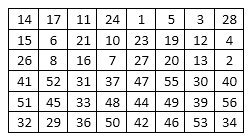
\includegraphics[scale=0.8]{Gambar/key_compression_matrix}
	%\centering
	%\caption{Matriks kompresi \textit{P-box}}
%\end{figure}

\section{Fungsi \textit{Hash}}
Fungsi \textit{hash} adalah algoritma kriptografi yang membuat kompresi dari pesan (\textit{message}) atau inti dari pesan, dimana kompresi ini dapat berfungsi sebagai \textit{fingerprint} atau disebut juga \textit{digest}. Fungsi \textit{hash} juga berfungsi untuk menjaga integritas sebuah pesan agar ketika ada perubahan pada pesan tersebut dapat langsung diketahui. Fungsi \textit{hash} akan memroses message (\textit{m}) menjadi \textit{message digest} atau \textit{digest} (\textit{h}). Bentuk umum dari fungsi \textit{hash}, yaitu:
\begin{displaymath}
	h = H(m)
\end{displaymath}

\noindent Fungsi \textit{hash} memiliki 4 kriteria utama, yaitu:
\begin{itemize}
	\item Semua nilai hash memiliki panjang yang sama.
	\item Mudah untuk menghitung nilai \textit{hash} untuk setiap \textit{message} masukkan.
	\item Nilai \textit{hash} tidak bisa dikembalikan menjadi \textit{message}.
	\item Tidak ada 2 atau lebih \textit{message} yang memiliki nilai \textit{hash} yang sama.
	\item Saat \textit{message} berubah maka nilai hashnya juga akan berubah.
\end{itemize}
Contoh fungsi \textit{hash} antara lain SHA-0, SHA-1, SHA-512, MD-2, dan MD-5.

\subsection{\textit{Secure Hashing Algorithm} 512 (SHA-512)}
\label{subsec:SHA512}
\textit{Secure hashing algorithm} 512 atau SHA-512 adalah algoritma fungsi \textit{hash} yang menghasilkan 512-\textit{bit} \textit{message digest}. SHA-512 merupakan algoritma fungsi \textit{hash} dalam versi SHA yang menghasilkan \textit{message digest} paling panjang (512-\textit{bit}). SHA-512 membuat 512-\textit{bit} digest yang diambil dari beberapa blok \textit{message}. Setiap blok \textit{message} panjangnya 1024 bit. Gambar di bawah ini menunjukkan cara pembuatan \textit{message digest}.

%diagram
\begin{figure}[ht]
	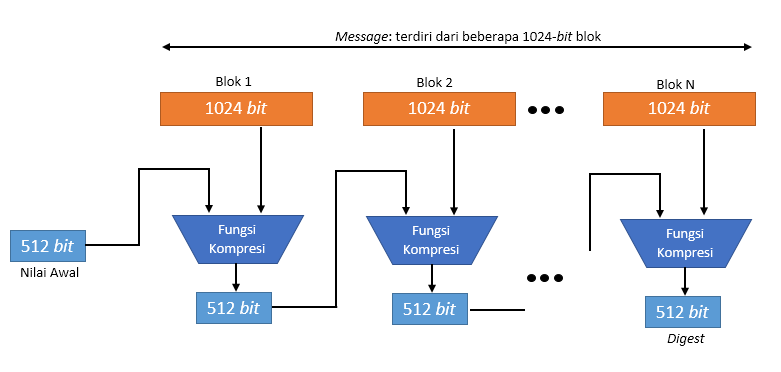
\includegraphics[scale=0.8]{Gambar/digest_creation}
	\centering
	\caption{Pembuatan \textit{message digest}}
\end{figure}

\subsubsection{Persiapan \textit{Message}}
\label{sssec:persiapan_message}
SHA-512 menerima masukan \textit{message} dengan panjang kurang dari \begin{math}2^{128}-\textit{bit}\end{math}, berarti jika panjang \textit{message} sama dengan \begin{math}2^{128}\end{math} atau lebih maka SHA-512 tidak memroses \textit{message} tersebut. Hal ini tidak akan menjadi masalah karena ukuran \begin{math}2^{128}-\textit{bit}\end{math} cukup besar untuk tempat penyimpanan komputer manapun.

\subsubsection{\textit{Length Field} dan \textit{Padding}}
Sebelum \textit{message digest} atau \textit{digest} dapat dibuat, SHA-512 membutuhkan tambahan 128-\textit{bit} yang menunjukkan panjang dari \textit{message}. Panjang dari \textit{message} ini direpresentasikan oleh 128-\textit{bit} tambahan.

%diagram
\begin{figure}[ht]
	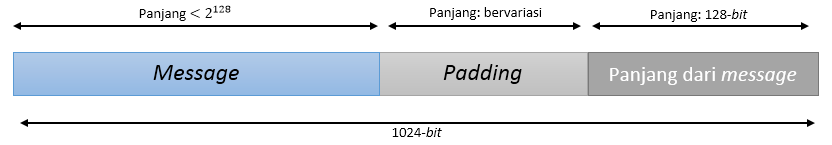
\includegraphics[scale=0.6]{Gambar/length_field_padding}
	\centering
	\caption{\textit{Length field} dan \textit{padding} dalam SHA-512}
\end{figure}

Sebelum menambahkan bagian 128-\textit{bit} yang menunjukkan panjang dari \textit{message} maka kita perlu melapisi (\textit{padding}) \textit{message} asli agar panjang totalnya bisa mencapai 1024-\textit{bit}. Panjang dari bagian \textit{padding} yang harus ditambahkan ini ditunjukkan dengan cara sebagai berikut, dengan \textit{P} adalah \textit{padding}, \textit{M} adalah \textit{message}.

\begin{displaymath}
	(M + P + 128) = 0\quad mod\quad 1024
\end{displaymath}

\begin{displaymath}
	P = (-M - 128)\quad mod\quad 1024
\end{displaymath}

Cara menuliskan \textit{padding} diawali dengan angka 1 kemudian diikuti oleh beberapa angka 0 (nol) sampai panjangnya mencapai \textit{P}.

\subsubsection{\textit{Words}}
SHA-512 beroperasi dengan ukuran \textit{words}. Panjang dari satu \textit{word} adalah 64-\textit{bit}. Ini berarti, setelah proses \textit{padding} ditambahkan pada \textit{message}, setiap blok \textit{message} akan terdiri dari 16 buah 64-\textit{bit word}. \textit{Message digest} atau \textit{digest} juga akan terdiri dari 64-\textit{bit word} namun panjangnya hanya 8 \textit{word} dan setiap \textit{word} nya dinamakan \begin{math}A, B, C, D, E, F, G\end{math}, dan \begin{math}H\end{math}.

%diagram
\begin{figure}[ht]
	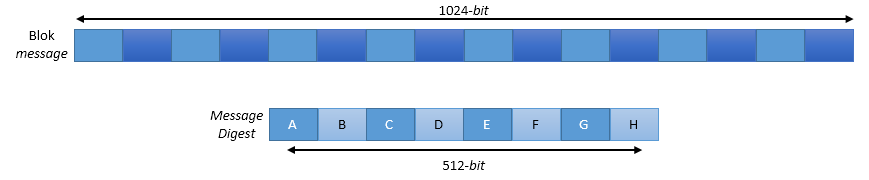
\includegraphics[scale=0.6]{Gambar/message_block_digest_as_words}
	\centering
	\caption{Blok \textit{message} dan \textit{message digest} dalam \textit{word}}
\end{figure}

\subsubsection{Ekspansi \textit{Word}}
\label{sssec:ekspansi_word}
Sebelum diproses, setiap blok \textit{message} harus diekspansi, panjang setiap blok ini adalah 1024-\textit{bit} terdiri dari 16 buah 64-\textit{bit word}. Pada tahap pemrosesan, dibutuhkan 80 buah 64-\textit{bit word} maka dari itu, 16 \textit{word} ini harus diekspansi menjadi 80 \textit{word}, \begin{math}W_0\end{math} sampai \begin{math}W_79\end{math}. Gambar di bawah ini akan menunjukkan cara ekspansi \textit{word}.

%diagram
\begin{figure}[ht]
	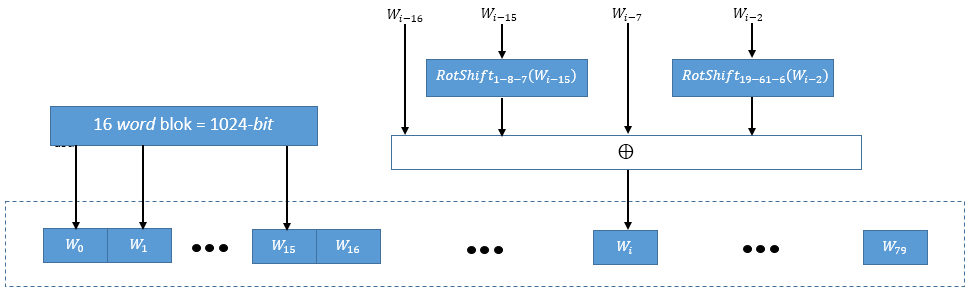
\includegraphics[scale=0.4]{Gambar/word_expansion}
	\centering
	\caption{Ekspansi \textit{word}}
\end{figure}

\begin{displaymath}
	RotShift_{l-m-n}(x):RotR_l(x) \oplus RotR_m(x) \oplus ShL_n(x)
\end{displaymath}

\noindent \begin{math}RotR_i(x)\end{math}: Rotasi ke kanan dari \begin{math}x\end{math} sebanyak \begin{math}i\end{math} \textit{bit}.\\
\begin{math}ShL_i(x)\end{math}: \textit{Shift left} \begin{math}x\end{math} sebanyak \begin{math}i\end{math} \textit{bit} ditambah (\textit{padding}) dengan 0.

\subsubsection{Inisialisasi \textit{Message Digest}}
SHA-512 menggunakan 8 buah konstanta dalam proses insialisasi \textit{message digest}. Konstanta ini akan diberi nama \begin{math}A_0\end{math} sampai \begin{math}H_0\end{math}. Setiap nilai dari konstanta didapat dari 8 bilangan prima pertama (2, 3, 5, 7, 11, 13, 17, 19). Setiap nilai merupakan nilai pecahan atau angka di belakang koma dari akar kuadrat bilangan prima yang bersangkutan.

Sebagai contoh, \begin{math}H_0\end{math} didapat dari nilai \begin{math}\sqrt{19} = 4.35889894354\end{math}. Kemudian, nilai ini akan dikonversi ke biner sepanjang 64-\textit{bit} maka akan diperoleh \begin{math}(100.0101\quad 1011\quad 1110 ... 1001)_2=(4.5BE0CD19137E2179)_{16}\end{math}. SHA-512 hanya mengambil nilai yang di belakang koma saja jadi nilai dari \begin{math}H_0 = 5BE0CD19137E2179\end{math}. Gambar di bawah ini menunjukkan nilai dari \begin{math}A_0\end{math} sampai \begin{math}H_0\end{math} dalam heksadesimal.

%diagram
\begin{figure}[ht]
	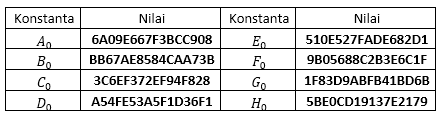
\includegraphics[scale=0.8]{Gambar/konstanta_sha}
	\centering
	\caption{Konstanta inisialisasi dalam SHA-512}\label{fig:konstanta_sha}
\end{figure}

\subsubsection{Fungsi Kompresi}
SHA-512 membuat \textit{message digest} sepanjang 512-\textit{bit} (8 \textit{word}) dari beberapa blok \textit{message} yang masing-masing panjangnya 1024-\textit{bit}. Pemrosesan setiap blok \textit{message} ini dilakukan sebanyak 80 ronde. Setiap ronde akan terdiri dari \begin{math}W_i\end{math} digabungkan dengan \begin{math}K_i\end{math} untuk membuat \begin{math}W_i\end{math} baru yang akan digunakan pada ronde selanjutnya. Pada akhir ronde 79, nilai \begin{math}W_0\end{math} sampai \begin{math}W_7\end{math} pada ronde 79 akan ditambahkan oleh nilai \begin{math}W_0\end{math} sampai \begin{math}W_7\end{math} pada ronde yang paling awal (ronde 0) dan dimodulo oleh \begin{math}2^{64}\end{math}. Hasil yang diperoleh disebut \textit{message digest} atau \textit{final digest}. Gambar di bawah ini menunjukkan proses fungsi kompresi pada SHA-512.

%diagram
\begin{figure}[ht]
	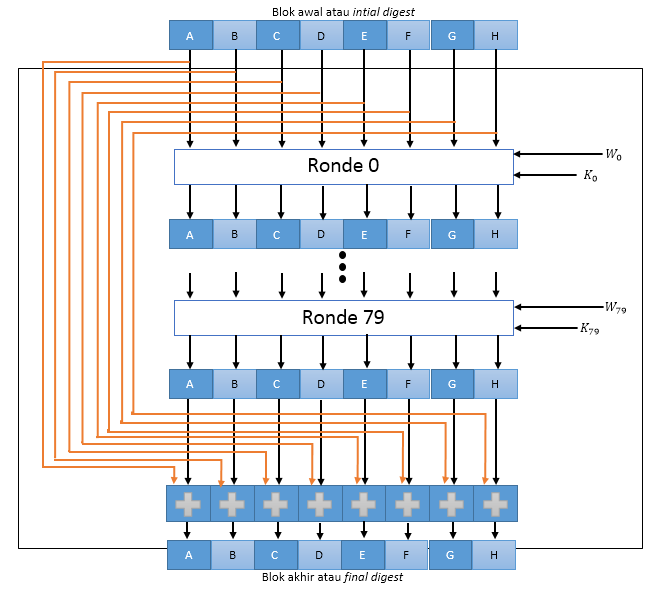
\includegraphics[scale=0.8]{Gambar/compression_function}
	\centering
	\caption{Fungsi kompresi dalam SHA-512}
\end{figure}

\subsubsection{Ronde}
\label{sssec:rondesha512}
Pada setiap ronde, 8 nilai baru pada 64-\textit{bit word} dibuat dari 8 nilai 64-\textit{bit word} pada ronde sebelumnya. Nilai baru ini dinamakan \textit{buffer}. Enam dari delapan \textit{buffer} mendapatkan nilai dari \textit{buffer} ronde sebelumnya. Sedangkan untuk 2 \textit{buffer} lagi nilai keduanya diperoleh dari sebuah fungsi kompleks yang berhubungan dengan \textit{buffer} sisanya serta gabungan tambahan dari \begin{math}W_i\end{math} dan \begin{math}K_i\end{math}, bersangkutan dengan masing-masing ronde. Gambar di bawah ini akan menjelaskan struktur dari setiap ronde serta fungsi kompleks yang digunakan untuk mendapatkan nilai untuk 2 \textit{buffer} (\begin{math}A\end{math} dan \begin{math}E\end{math}).

%diagram
\begin{figure}[ht]
	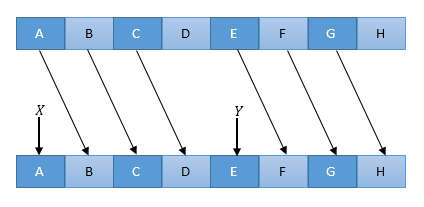
\includegraphics[scale=0.8]{Gambar/sha_round}
	\centering
	\caption{Struktur ronde dalam SHA-512}
\end{figure}

%diagram
\begin{figure}[ht]
	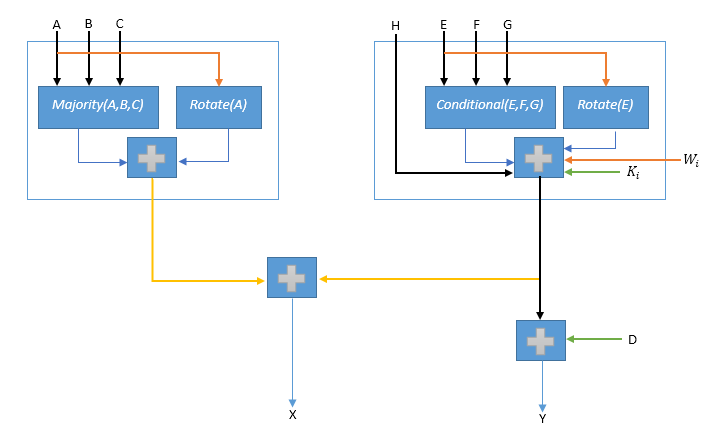
\includegraphics[scale=0.7]{Gambar/complex_function}
	\centering
	\caption{Fungsi kompleks dalam SHA-512}
\end{figure}

Nilai dari \begin{math}Majority(A, B, C)\end{math}, \begin{math}Conditional(E, F, G)\end{math}, \begin{math}Rotate(A)\end{math}, dan \begin{math}Rotate(E)\end{math} pada gambar di atas didapat dari rumus di bawah ini.
\begin{displaymath}
	Majority(x,y,z) = (x\: AND\: y)  \oplus (y\: AND\: z) \oplus (z\: AND\: x)
\end{displaymath}

\begin{displaymath}
	Conditional(x,y,z) = (x\: AND\: y)  \oplus (NOT\: x\: AND\: z) 
\end{displaymath}

\begin{displaymath}
	Rotate(x) = RotR_{28}(x) \oplus RotR_{34}(x) \oplus RotR_{39}(x) 
\end{displaymath}

\begin{math}RotR_i(x)\end{math} adalah rotasi ke kanan \begin{math}x\end{math} sebanyak \begin{math}i\end{math} \textit{bit}. Simbol kotak yang berisi tanda tambah berarti adalah penambahan antar \textit{bit-bit} lalu kemudian hasilnya di modulo oleh \begin{math}2^{64}\end{math}. \begin{math}K_i\end{math} pada fungsi kompleks diatas didapat dengan cara yang sama saat mencari nilai dari konstanta awal \begin{math}A_0\end{math} sampai \begin{math}H_0\end{math}. Namun, karena yang digunakan sebanyak 80 buah dari \begin{math}K_0\end{math} sampai \begin{math}K_{79}\end{math} maka banyak bilangan prima yang digunakan juga sebanyak 80 bilangan prima pertama mulai dari 2 sampai 409.

Perbedaannya dengan nilai dari konstanta awal adalah nilai \begin{math}K_i\end{math} pada fungsi kompleks didapat dari akar kubik bilangan prima yang bersangkutan. Selanjutnya, proses yang sama dengan cara menentukan nilai konstanta awal tetap digunakan untuk menentukan nilai \begin{math}K_i\end{math}. Sebagai contoh, \begin{math}\sqrt[3]{409} = 7.42291412044\end{math}, kemudian akan dikonversi ke dalam biner menjadi \begin{math}(111.0110\: 1100\: 0100\: 0100\: ... 0111)_2\end{math} dan dikonversi ke dalam heksadesimal menjadi \begin{math}(7.6C44198C4A475817)_{16}\end{math}, kemudian nilai yang diambil hanya nilai di belakang koma, maka nilai dari \begin{math}K_{79} = 6C44198C4A475817\end{math}.

\section{Otentikasi}
Otentikasi adalah proses untuk menentukan apakah sebuah entitas diijinkan untuk mengakses sumber daya yang dimiliki sebuah sistem. Otentikasi juga merupakan proses untuk memastikan keaslian data. Otentikasi dibagi menjadi 2 jenis, yaitu:

\subsection{Otentikasi Pesan (\textit{Message Authentication})}
Sebuah pesan inti (\textit{message digest}) dapat digunakan untuk menjamin integritas sebuah pesan, memastikan pesan tidak diubah. Namun, pesan inti tidak bisa memastikan keaslian pengirim pesan. Ketika Alice mengirim pesan kepada Bob, Bob harus bisa tahu bahwa pesan yang dikirim berasal dari Alice. Supaya Bob bisa memastikan bahwa Alice yang mengirim pesan, maka Alice harus bisa menyediakan bukti bahwa Alice adalah pengirimnya. Contoh dari otentikasi ini antara lain adalah \textit{modification detection code} (MDC) dan \textit{message authentication code} (MAC).

\subsubsection{\textit{Modification Detection Code}}
\textit{Modification detection code} merupakan sebuah pesan inti yang dapat memastikan integritas dari sebuah pesan, bahwa pesan tidak diubah saat proses pengiriman. Alice dapat membuat pesan inti, yaitu kode deteksi modifikasi dan mengirimkannya bersama dengan pesan asli kemudian Bob akan membuat juga secara terpisah kode deteksi modifikasi berdasarkan pesan asli yang dikirim Alice dan membandingkan dengan kode deteksi modifikasi yang dikirim Alice. Jika sama, maka pesan yang dikirim oleh Alice asli dan tidak berubah saat pengiriman. Proses diatas dapat ditunjukkan pada diagram di bawah ini.

%diagram
\begin{figure}[ht]
	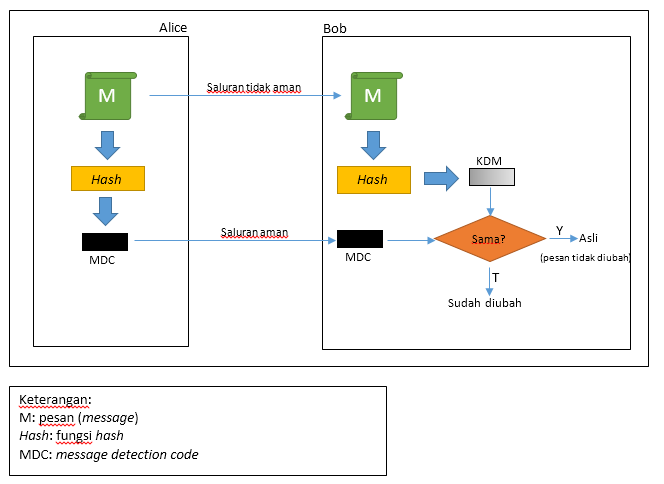
\includegraphics[scale=0.65]{Gambar/MDC}
	\centering
	\caption{\textit{Modification detection code}}
\end{figure}

Diagram diatas menunjukkan bahwa pesan yang dikirim Alice dapat dikirim melalui saluran yang tidak aman, maksudnya pihak lain diluar Alice dan Bob bisa membacanya bahkan mengubah isinya, tapi MDC yang dibuat oleh Alice harus dikirimkan pada Bob di saluran aman. Dengan cara ini, MDC tidak akan bisa diubah isinya dan ketika pesan yang dikirim melalui saluran tidak aman diubah maka Bob akan tahu bahwa pesan sudah diubah oleh pihak lain dengan membandingkan hasil MDC dari pesan yang dia terima dengan MDC yang Alice kirimkan melalui saluran aman.

\subsubsection{\textit{Message Authentication Code}}
Untuk memastikan bahwa memang Alice yang mengirimkan pesan kepada Bob maka kode deteksi pesan yang digunakan harus diubah menjadi \textit{message authentication code} (MAC). Perbedaan MAC dengan MDC adalah MAC menggunakan sebuah kunci rahasia atau kunci pribadi yang hanya diketahui oleh Alice dan Bob saja. Diagram di bawah ini akan menunjukkan cara kerja MAC dalam mengotentikasi pesan.

%diagram
\begin{figure}[ht]
	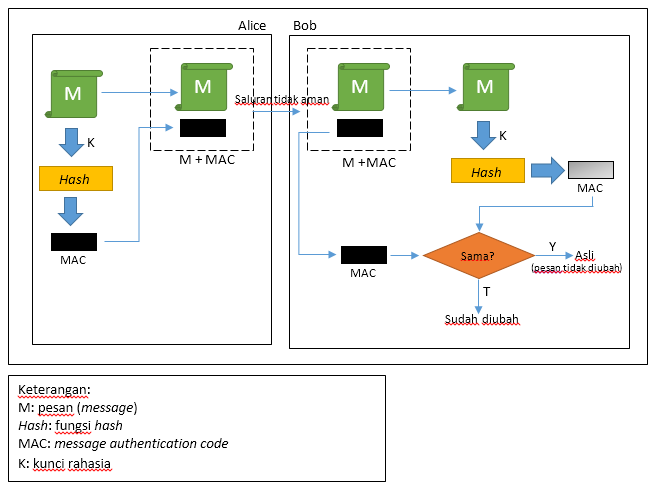
\includegraphics[scale=0.7]{Gambar/MAC}
	\centering
	\caption{\textit{Modification authentication code}}
\end{figure}

Alice menggunakan fungsi \textit{hash} untuk membuat MAC dengan menggunakan gabungan dari pesan dan kunci rahasia yang hanya diketahui olehnya dan Bob saja. Kemudian, Alice mengirimkan pesan beserta dengan MAC pesan tersebut kepada Bob. Bob akan menerima pesan dan memisahkan MAC dengan pesan dan kemudian Bob akan membuat MAC dari pesan yang diterima dari Alice dengan menggunakan fungsi hash yang sama seperti Alice gunakan dan tentu saja MAC yang dibuat merupakan gabungan dari pesan dan kunci rahasia. Melalui cara ini, jika hasil keluaran MAC yang Bob buat sendiri dibandingkan dengan MAC yang Alice kirimkan sama, maka Bob bisa yakin dengan pasti bahwa pesan yang dia terima berasal dari Alice dan pesan tersebut asli, tidak diubah oleh pihak lain. Terdapat beberapa modifikasi dari \textit{message authentication code} antara lain adalah \textit{nested MAC}, \textit{hashed MAC}, dan CMAC. 

\subsection{Otentikasi Entitas (\textit{Entity Authentication})}
Otentikasi entitas merupakan sebuah teknik yang dirancang untuk memastikan kebenaran identitas seseorang. Entitas yang dimaksud disini bisa berupa orang, pengguna (\textit{user}), atau sebuah \textit{server}. Entitas yang identitasnya perlu dibuktikan kebenarannya disebut penuntut (\textit{claimant}) dan entitas yang bertindak untuk memastikan kebenaran identitas dari penuntut disebut pemeriksa (\textit{verifier}). Ketika Bob hendak memastikan kebenaran identitas dari Alice, Bob adalah pemeriksa dan Alice adalah penuntut.

Ada dua perbedaan antara otentikasi pesan dan otentikasi entitas:
\begin{enumerate}
	\item Otentikasi pesan atau otentikasi sumber data tidak terjadi secara langsung sedangkan otentikasi entitas terjadi secara langsung.
	\item Otentikasi pesan hanya mengotentikasi satu pesan saja, ketika pesan berikutnya dikirimkan maka proses otentikasi pesan akan dilakukan kembali sedangkan otentikasi entitas akan terjadi selama satu durasi dalam sebuah sesi.
\end{enumerate}

Dalam otentikasi entitas, penuntut harus bisa membuktikan kebenaran identitas dirinya kepada pemeriksa. Ada beberapa cara pembuktian yang bisa dilakukan oleh penuntut, yaitu:
\begin{itemize}
	\item Sesuatu yang diketahui (\textit{something known}). Hal ini diketahui oleh penuntut dan juga pemeriksa. Contohnya antara lain adalah \textit{password}, nomor PIN, kunci rahasia, dan kunci pribadi.
	\item Sesuatu yang dimiliki (\textit{something possessed}). Hal ini dimiliki oleh penuntut dan bisa memastikan kebenaran identitas dari penuntut. Contohnya antara lain adalah paspor, KTP, kartu kredit, dan SIM.
	\item Sesuatu yang melekat (\textit{something inherent}). Hal ini menempel atau sebagai bagian dari penuntut. Contohnya antara lain adalah sidik jari, suara, tanda tangan, pola retina, dan tulisan tangan.
\end{itemize}

\begin{flushleft}
	Beberapa teknik dalam otentikasi entitas antara lain, yaitu \textit{password}, \textit{zero-knowledge}, \textit{challenge-response}, dan biometrik.
\end{flushleft}

\subsection{\textit{Password}}
Salah satu teknik otentikasi entitas yang paling sederhana dan mudah adalah otentikasi menggunakan \textit{password} atau kata kunci rahasia. \textit{Password} ini adalah sesuatu yang diketahui hanya oleh penuntut. \textit{Password} digunakan saat penuntut (selanjutnya akan dinamakan pengguna) perlu untuk mengakses sistem untuk menggunakan sumber daya dari sistem. Setiap pengguna akan diberikan \textit{username} yang sifatnya publik dan \textit{password} yang sifatnya rahasia atau pribadi. Ada dua skema otentikasi menggunakan \textit{password} ini, yaitu \textit{password} tetap (\textit{fixed password}) dan \textit{password} satu-kali (\textit{one-time password}).

\subsubsection{\textit{Password} Satu-Kali}
\textit{Password} satu-kali adalah \textit{password} yang digunakan hanya satu kali. Jadi, setiap kali pengguna akan mengakses sistem untuk setiap sesi waktu yang berbeda, maka \textit{password} yang digunakan akan selalu berbeda-beda. Beberapa teknik yang digunakan dalam \textit{password} satu-kali antara lain menggunakan \textit{list}, \textit{sequentially updated password}, dan \textit{password} satu-kali \textit{lamport}.

\subsubsection{\textit{Password} Tetap}
\textit{Password} tetap (\textit{fixed password}) adalah \textit{password} yang digunakan berulang-ulang kali setiap saat pengguna akan mengakses sistem. \textit{Password} ini akan selalu sama untuk setiap kali pengguna akan mengakses sistem. Ada beberapa skema dari \textit{password} tetap ini.

\begin{itemize}
	\item Skema 1\\
	Dalam skema ini, sistem menyimpan setiap \textit{password} dalam sebuah tabel basis data yang diurutkan berdasarkan nama pengguna (\textit{username}). Saat pengguna akan mengakses sistem, maka pengguna akan memasukkan \textit{username} dan \textit{password} dalam bentuk \textit{plaintext}. Kemudian, sistem akan mencari \textit{password} berdasarkan \textit{username}. Jika \textit{password} yang dimasukkan pengguna sesuai dengan \textit{password} yang ada dalam tabel basis data maka pengguna diberikan akses masuk ke dalam sistem, jika tidak sesuai maka pengguna tidak diberikan akses masuk ke dalam sistem. Kekurangan dari skema ini adalah karena \textit{password} disimpan dalam tabel basis data maka setiap orang yang memiliki akses ke dalam basis data dapat mengetahui setiap \textit{password} yang disimpan dan tentu saja hal ini melanggar salah satu layanan dari kriptografi yaitu, kerahasiaan data (\textit{data confidentiality}).
	% diagram
	\begin{figure}[ht]
		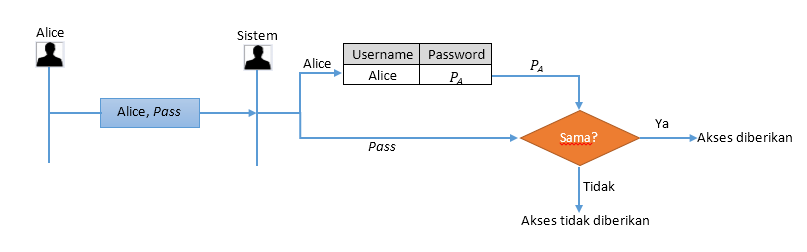
\includegraphics[scale=0.7]{Gambar/password_1}
		\centering
		\caption{\textit{Username} dan \textit{Password}}
	\end{figure}
	
	\item Skema 2\\
	Skema yang lebih aman dibandingkan skema diatas adalah skema penyimpanan password yang menggunakan fungsi \textit{hash}. Sistem tidak lagi menyimpan \textit{password} dengan bentuk \textit{plaintext} dalam tabel basis data, namun sistem menyimpan \textit{password} dalam bentuk hashnya dalam tabel basis data, sehingga saat sistem dibobol maka penyerang tidak dapat mengetahui \textit{password} secara langsung karena fungsi \textit{hash} adalah fungsi satu arah dan mustahil untuk mengembalikan ke \textit{plaintext}nya. Selain itu, orang-orang yang memiliki akses ke dalam basis data tidak bisa mengetahui \textit{password} dari setiap \textit{username} yang disimpan dalam tabel. Ketika \textit{password} dibuat, sistem akan menghitung nilai \textit{hash} dari \textit{password} dan menyimpan nilai hash tersebut dalam tabel basis data.
Saat pengguna akan mengakses sistem, pengguna memasukkan \textit{username} dan \textit{password} dalam bentuk \textit{plaintext} kemudian sistem akan menghitung nilai hash dari \textit{password} tersebut dan menyesuaikan dengan nilai \textit{hash} dari \textit{password} yang bersangkutan dalam tabel basis data. Jika sesuai, maka pengguna diberikan ijin masuk ke dalam sistem, jika tidak maka pengguna tidak diberikan ijin masuk.
	% diagram
	\begin{figure}[ht]
		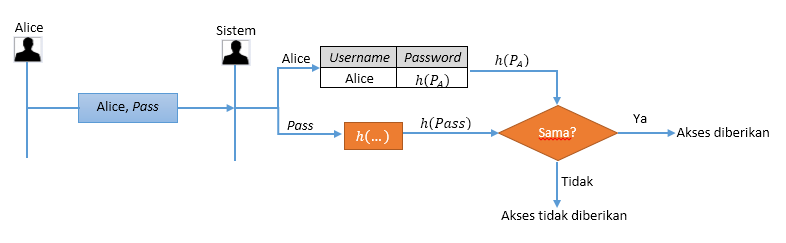
\includegraphics[scale=0.7]{Gambar/password_2}
		\centering
		\caption{\textit{Password hashing}}
	\end{figure}
	
	\item Skema 3\\
	Skema ketiga menggunakan teknik \textit{salting}. Ketika \textit{password} dibuat, sebuah \textit{string} acak, disebut \textit{salt}, akan ditambahkan pada \textit{password}. Setelah ditambahkan, \textit{password} yang bersangkutan akan dihitung nilai \textit{hash}nya. Sistem akan menyimpan \textit{username}, \textit{salt}, dan \textit{hash} atau \textit{digest} dari \textit{password} dalam tabel basis data. Ketika pengguna akan mengakses sistem, sistem akan mengambil \textit{salt} berdasarkan \textit{username} yang dimasukkan kemudian menambahkan \textit{salt} tersebut pada \textit{password} yang dimasukkan dan menghitung nilai \textit{hash}nya kemudian menyesuaikan dengan yang ada pada tabel basis data. Jika sesuai, maka akses diberikan, jika tidak maka akses akan ditolak.
		% diagram
	\begin{figure}[ht]
		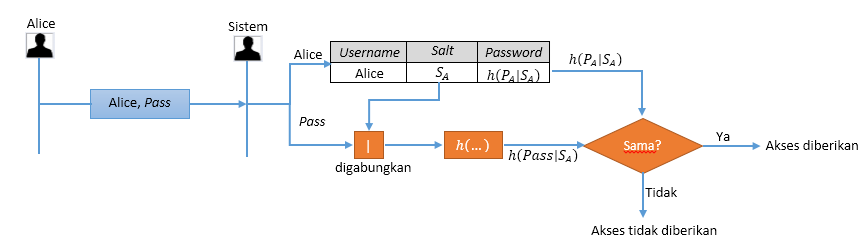
\includegraphics[scale=0.5]{Gambar/password_3}
		\centering
		\caption{\textit{Password salting}}
	\end{figure}
\end{itemize}

\section{\textit{Secret Sharing}}
Enkripsi digunakan untuk menjaga keamanan informasi dan setiap proses enkripsi disertai oleh sebuah kunci rahasia atau \textit{password}. \textit{Password} ini tentu saja harus selalu diingat oleh manusia atau disimpan dalam memori komputer. Namun, hal ini tidak sepenuhnya aman karena bisa saja manusia lupa atau terjadi kerusakan komputer atau bencana alam sehingga \textit{password} ini hilang dan informasi yang dienkripsi tidak akan bisa diakses atau dikembalikan.

\textit{Secret sharing} adalah metode untuk membagi informasi (rahasia) menjadi beberapa bagian. Bagian-bagian tersebut disebut \textit{share} dan setiap bagian dibagikan kepada beberapa partisipan. Untuk mendapatkan kembali informasi, maka dibutuhkan sejumlah \textit{share}.

Shamir mendasarkan metode \textit{secret sharing} dalam sebuah masalah sebagai berikut:
\begin{center}
''\textit{Sebelas orang ilmuwan mengerjakan sebuah projek rahasia. Mereka menyimpan dokumen dalam sebuah kabinet dimana kabinet ini hanya akan bisa dibuka jika enam atau lebih ilmuwan hadir. Berapa banyak kunci minimal yang dibutuhkan untuk membuka kabinet? Berapa banyak kunci yang harus dimiliki oleh masing-masing ilmuwan?}''
\end{center}

Tentu saja jawabannya minimal sebanyak 462 kunci untuk membuka kabinet dan minimal 252 kunci yang harus dimiliki oleh setiap ilmuwan. Angka ini sangat tidak masuk akal dan menyulitkan apalagi jika banyak ilmuwannya bertambah.
Dalam skema \textit{secret sharing} shamir, suatu data \textit{D} akan dibagi menjadi \textit{n} buah \textit{share} dengan ketentuan sebagai berikut:
	\begin{itemize}
		\item Jika bagian yang ada sebanyak \textit{k} bagian atau lebih akan membuat \textit{D} mudah untuk dibentuk kembali.
		\item Jika bagian yang ada hanya sebanyak \textit{k-1} atau kurang maka \textit{D} tidak akan dapat dibentuk kembali.
\end{itemize}
Skema diatas dinamakan skema \textit{threshold}(\textit{k},\textit{n}).

\subsection{Skema \textit{Threshold}(\textit{k},\textit{n})}
Enkripsi dilakukan untuk melindungi kerahasiaan sebuah data atau informasi, namun karena setiap proses enkripsi memerlukan kunci maka diperlukan cara lain untuk melindungi kerahasiaan kunci tersebut. Salah satu cara yang paling aman dalam melindungi kunci kriptografi adalah dengan menyimpannya dalam sebuah lokasi yang aman dan tersembunyi (komputer, otak manusia, atau lemari besi).

Namun cara ini tidak sepenuhnya aman karena bisa saja terjadi bencana alam, kematian, penipuan dan sabotase menyebabkan kunci yang disimpan menjadi rusak atau hilang sehingga data yang dienkripsi menjadi tidak bisa diakses dan hilang sepenuhnya. Solusi lainnya adalah dengan memperbanyak kunci yang ada dan menyimpannya di tempat yang berbeda-beda, satu di memori komputer, satu diingat oleh manusia, dan yang lainnya disimpan di tempat yang berbeda-beda. Namun, cara ini juga tidak aman karena masih tidak terhindar dari bencana alam, \textit{human error}, dan malapetaka lainnya.

Untuk mengatasi permasalahan ini maka dibutuhkan sebuah mekanisme atau skema, skema tersebut dinamakan skema \textit{threshold}(\textit{k},\textit{n}). Skema \textit{threshold(k,n)} didasarkan pada interpolasi polinomial: diberikan k titik pada bidang kartersius \begin{math}(x_1,y_1), (x_2, y_2), ...,(x_k, y_k)\end{math} untuk setiap \begin{math}x_i\end{math} maka hanya akan ada 1 saja nilai \begin{math}q(x_i)\end{math} dalam derajat \begin{math}k-1\end{math} dimana \begin{math}q(x_i)=y_i\end{math} untuk seluruh \begin{math}x_i\end{math}. Misalkan diasumsikan bahwa \textit{D} adalah representasi berupa angka dari kunci yang akan dipecah menjadi beberapa bagian atau \textit{share} menggunakan skema \textit{threshold(k,n)}, kemudian untuk membagi \textit{D} menjadi \begin{math}D_i\end{math} \textit{share}, dipilih \begin{math}k-1\end{math} derajat polinomial untuk membentuk fungsi \begin{math}q(x)\end{math}:
\begin{displaymath}
	q(x) = a_0 + a_1 * x + a_2 * x^2 + ... + a_{k-1} * x^{k-1}
\end{displaymath}
\begin{displaymath}
	a_0 = D
\end{displaymath}

Nilai \begin{math}a_1\end{math} sampai \begin{math}a_{k-1}\end{math} dipilih secara acak kemudian dihitung nilai dari \begin{math}D_1\end{math} sampai \begin{math}D_n\end{math} dimana \begin{math}n\end{math} adalah banyaknya \textit{share}:

\begin{displaymath}
	D_1 = q(1), D_2 = q(2), ... , D_i = q(i), ... , D_n = q(n)
\end{displaymath}

Untuk setiap nilai dari \begin{math}D_n\end{math} yang diketahui, maka bisa dicari nilai koefesien dari fungsi \begin{math}q(x)\end{math} dengan interpolasi atau penyelesaian sistem persamaan linear, dari situ bisa diperoleh nilai dari \begin{math}q(0)\end{math} sehingga nilai \textit{D} nanti bisa diketahui. Namun, \textit{D} bisa dihitung jika \textit{k} atau lebih \textit{share} diketahui, jika hanya \begin{math}k-1\end{math} atau kurang \textit{share} yang diketahui, maka nilai \textit{D} tidak bisa dihitung sehingga data tidak bisa dikembalikan.

Namun, dengan nilai \textit{k} yang tinggi juga akan sulit untuk mendapatkan data, karena banyak \textit{share} yang dikumpulkan. Dengan mengurangi nilai \textit{k}, akan mempermudah untuk mendapatkan kembali data sehingga mengatasi akibat atau hilangnya beberapa \textit{share}. Pemilihan \textit{k} dan \textit{n} yang tepat dapat menjaga kerahasiaan data.

\section{Probabilitas}
Probabilitas atau peluang merupakan salah cara dalam ilmu matematika untuk mengukur tingkat kepercayaan akan suatu kejadian. Teori probabilitas sangat luas penggunaannya, baik dalam kehidupan sehari-hari maupun dalam percobaan-percobaan ilmiah. Teori probabilitas ini seringkali digunakan oleh para pengambil keputusan untuk memprediksi suatu kejadian sehingga nantinya bisa mengambil keputusan yang tepat.

Seluruh kemungkinan keluaran yang akan terjadi dalam probabilitas disebut ruang sampel sedangkan masing-masing kemungkinan yang dapat terjadi dalam ruang sampel dinamakan elemen atau anggota dari ruang sampel. Ruang sampel dilambangkan dengan huruf \begin{math}S\end{math} dan elemen dilambangkan dengan huruf \begin{math}x_i\end{math}. Dalam notasi matematikanya:

\begin{displaymath}
	S = {x_1, x_2, x_3, ..., x_n}
\end{displaymath}

Sedangkan probabilitas akan kemungkinan bahwa kejadian \begin{math}x_i\end{math} akan terjadi dilambangkan dengan \begin{math}P(x_i)\end{math}. Dalam rumus matematikanya:

\begin{displaymath}
	P(x_i) = \frac{n}{N}
\end{displaymath}

\noindent dimana \begin{math}n\end{math} adalah banyaknya kemunculan kejadian \begin{math}x_i\end{math} dalam sebuah ruang sampel \begin{math}S\end{math} dan \begin{math}N\end{math} adalah banyaknya kejadian yang terjadi dalam ruang sampel \begin{math}S\end{math}.

\section{Distribusi Binom}
Setiap eksperimen atau percobaan yang dilakukan secara berkali-kali pasti memiliki dua keluaran, yaitu sukses atau gagal. Untuk setiap keluaran yang diperoleh (baik sukses maupun gagal) bisa ditetapkan sebagai sukses. Proses ini dinamakan proses bernouli dan setiap eksperimen yang dilakukan untuk setiap proses bernouli dinamakan percobaan bernouli. Ada beberapa syarat sebuah eksperimen bisa dinamakan percobaan bernouli:
\begin{enumerate}
	\item Eksperimen harus diulang sebanyak \begin{math}n\end{math} kali.
	\item Setiap keluaran dari perulangan bisa dianggap sukses atau gagal.
	\item Probabilitas bahwa keluarannya sukses, \begin{math}p\end{math}, harus selalu sama untuk setiap kali perulangan.
	\item Setiap perulangan tidak dipengaruhi dengan perulangan sebelumnya atau independen.
\end{enumerate}

Maka, untuk banyak perulangan yang sukses, \begin{math}X\end{math}, dalam \begin{math}n\end{math} perulangan percobaan bernouli dinamakan variabel acak binom sedangkan untuk probabilitas dari variabel acak ini dinamakan distribusi binom dilambangkan dengan \begin{math}P(x,n,p)\end{math}, dimana \begin{math}p\end{math} merupakan probabilitas keluaran sukses dan \begin{math}1-p\end{math}, yaitu \begin{math}q\end{math} merupakan probabilitas keluaran gagal. Karena percobaan dilakukan sebanyak \begin{math}n\end{math} kali maka probabilitas keseluruhannya menjadi \begin{math}p^n q^{(n-x)}\end{math}, kemudian karena sebanyak \begin{math}x\end{math} kejadian sukses yang diambil dari keseluruhan ruang sampel \begin{math}n\end{math}, maka probabilitas \begin{math}p\end{math} dan \begin{math}q\end{math} akan dikalikan dengan kombinasi \begin{math}n\end{math} dan \begin{math}x\end{math}, dituliskan menjadi \begin{math}\left( {\begin{array}{c}n \\ x \end{array}} \right)\end{math}. Jadi, dalam notasi matematikanya:

\begin{displaymath}
	P(x,n,p) = \left( {\begin{array}{c}n \\ x \end{array}} \right) p^n q^{(n-x)}
	\qquad\qquad
	%\quad\quad
	x = 0, 1, 2, ..., n
\end{displaymath}

\section{Entropi}
Entropi adalah rata-rata banyak informasi yang dimiliki oleh sebuah pesan. Pesan yang dimaksud disini adalah kejadian yang diharapkan atau elemen dari sebuah ruang sampel atau kejadian. Maka dari itu, entropi bisa dijadikan alat ukur dari tingkat ketidakpastian yang dimiliki oleh sebuah pesan atau sumber informasi. Misalkan sebuah pesan \begin{math}X\end{math} terdiri dari huruf-huruf. Untuk setiap huruf \begin{math}x\end{math} yang ada dalam pesan \begin{math}X\end{math} memiliki banyak kemunculan \begin{math}n\end{math} dan \begin{math}X\end{math} terdiri dari huruf-huruf sebanyak \begin{math}N\end{math}. Kemudian untuk setiap huruf yang bukan \begin{math}x\end{math}, \begin{math}y\end{math}, memiliki banyak kemunculan \begin{math}m\end{math}. Maka, nilai entropi yang dimiliki oleh pesan \begin{math}X\end{math} untuk huruf \begin{math}x\end{math}, \begin{math}H(x)\end{math}:

\begin{displaymath}
	H(x) = -\frac{n}{N}\log_2 (\frac{n}{N}) - \frac{m}{N}\log_2 (\frac{m}{N}) 
\end{displaymath}

\noindent atau untuk setiap huruf \begin{math}x\end{math} dalam pesan \begin{math}X\end{math}, probabilitas kemunculannya adalah \begin{math}p\end{math} dan untuk setiap huruf bukan \begin{math}x\end{math} dalam pesan \begin{math}X\end{math} probabilitas kemunculannya adalah \begin{math}q\end{math}, sehingga rumus nilai entropinya menjadi:

\begin{displaymath}
	H(x) = -p\log_2 p - q\log_2 q
\end{displaymath}

\noindent dimana \begin{math}q = 1-p\end{math} dan menggunakan logaritma basis 2 karena probabilitas kemunculannya biner, yaitu huruf \begin{math}x\end{math} dan huruf bukan \begin{math}x\end{math}.